\documentclass[11pt, a4paper]{article}
\usepackage[utf8]{inputenc}
\usepackage{amsmath,setspace,geometry}
\usepackage{amsthm}
\usepackage{amsfonts}
\usepackage{mathtools}
\mathtoolsset{showonlyrefs}
\usepackage[shortlabels]{enumitem}
\usepackage{rotating}
\usepackage{pdflscape}
\usepackage{graphicx}
\usepackage{bbm}
\usepackage[dvipsnames]{xcolor}
\usepackage[colorlinks=true, linkcolor= RawSienna, citecolor = RawSienna, filecolor = RawSienna, urlcolor = RawSienna, hypertexnames = true, backref = page]{hyperref}
\usepackage[]{natbib} 
\bibpunct[:]{(}{)}{,}{a}{}{,}
\geometry{left = 1.0in,right = 1.0in,top = 1.0in,bottom = 1.0in}
\usepackage[english]{babel}
\usepackage{float}
\usepackage{caption}
\usepackage{subcaption}
\usepackage{tikz}
\usepackage{booktabs}
\usepackage{pdfpages}
\usepackage{threeparttable}
\usepackage{framed}
\usepackage{comment}
\usepackage{lscape}
\usepackage{bm}
\setstretch{1.4}
%\usepackage[tablesfirst,nolists]{endfloat}

\usepackage[T1]{fontenc}
\usepackage{mlmodern}  % 太いComputer Modern
% MLmodernのバグを修正: cf. https://tex.stackexchange.com/questions/646333/size-of-integral-symbol-in-section-header-with-mlmodern
\DeclareFontFamily{OMX}{mlmex}{}
\DeclareFontShape{OMX}{mlmex}{m}{n}{<->mlmex10}{} 
\usepackage{tgtermes} % 数式以外の欧文をTXフォントで上書き

\newtheorem{theorem}{Theorem}
\newtheorem{assumption}{Assumption}
\newtheorem{lemma}{Lemma}
\newtheorem{definition}{Definition}
\newtheorem{proposition}{Proposition}
\newtheorem{claim}{Claim}
\newtheorem{corollary}{Corollary}
\newtheorem{example}{Example}
\DeclareMathOperator{\rank}{rank}

\theoremstyle{remark}
\newtheorem{remark}{Remark}

\title{Note on the identification of conduct parameters in homogeneous goods markets}
\author{Yuri Matsumura\thanks{\href{mailto:}{yuri.matsumura23@gmail.com}, Department of Economics, Rice University.} \and Suguru Otani \thanks{\href{mailto:}{suguru.otani@e.u-tokyo.ac.jp}, Market Design Center, Department of Economics, University of Tokyo
\\Declarations of interest: none %this is for Economics Letters
}}

\begin{document}

\maketitle
\begin{abstract}
    In this note, we revisit the identification result of conduct parameters in homogeneous goods markets by \citet{lau1982identifying}.
    The result is that the conduct parameter cannot be identified if and only if the demand function is separable but not a specific functional form.
    We show that the result is incorrect by providing a separable demand function that induces identification.
    This implies that the class of inverse demand functions that lead to identification is broader than \citet{lau1982identifying} considers.
    Therefore, when the market has enough variation, the conduct parameter can be identified in the broader class of inverse demand functions.
\end{abstract}

\noindent\textbf{Keywords:} Conduct parameters, Homogenous Goods Market
\vspace{0in}
\newline
\noindent\textbf{JEL Codes:} C5, C13, L1

\bigskip





\section{Introduction}
Measuring competitiveness is an important task in the empirical industrial organization literature.
The conduct parameter approach is one of the useful approaches to measure competitiveness.
However, the parameter cannot be directly measured from data because data generally lack information about marginal costs.
Therefore, researchers endeavor to identify and estimate conduct parameters.

In homogeneous goods markets, \cite{bresnahan1982oligopoly} considers the identification of the conduct parameter and the marginal cost function in linear demand and linear marginal cost model.
\citet{bresnahan1982oligopoly} finds that when the researcher can obtain a demand shifter, called a demand rotation instrument, that changes the slope and intercept of the inverse demand function, the conduct parameter and the marginal cost parameter can be identified.
Recently, \citet{matsumura2023resolving} provide a detailed condition for the identification.
\citet{lau1982identifying} considers a more general setting and shows that the conduct parameter is not identified if and only if the demand function is separable, except a specific functional form.

However, we show that the identification result in \citet{lau1982identifying} is incorrect by providing a counterexample where a separable demand function induces identification.
While the proof of \citet{lau1982identifying} is incorrect, we don't need to worry because the counterexample shows that the class of inverse demand functions that lead to identification is broader than the class considered in \citet{lau1982identifying}.
Thus, when the market has enough variation, the conduct parameter can be identified in a broader class of inverse demand functions.


\section{Model}
Consider a homogeneous product market with the aggregate inverse demand and aggregate marginal cost function as $P(Q, X^{d})$ and $MC(Q, X^{s})$ where $X^{d}$ and $X^{s}$ are the vector of exogenous variables.
Assume that $X^{d}$ and $X^{s}$ are exclusive; that is, there is no common variable in $X^{d}$ and $X^{s}$.
Thus, $X^{d}$ works as demand shifters, and $X^{s}$ works as cost shifters. 
Let $K_d$ and $K_s$ be the number of demand shifters and cost shifters, respectively.
The equilibrium quantity is characterized by the first-order condition
 \begin{align}
    P(Q, X^{d}) + \theta \frac{\partial P}{\partial Q}(Q, X^{d})Q &= MC(Q, X^{s}),
\end{align}
where $\theta$ is called the conduct parameter. 
Depending on the value of $\theta$, the relation can nest the first-order condition of several models, such as perfect competition ($\theta=0$) and Cournot competition ($\theta=1/N$). 
See the Appendix for the details of the interpretation.


Suppose that the researcher observes the aggregate price $P$ and the aggregate quantity $Q$, and the vector of exogenous variables $X^{d}$ and $X^{s}$.
In this setting, the researcher can independently identify the inverse demand function by using the demand and cost shifters.
Therefore, the researcher wants to identify the conduct parameter and the marginal cost function from the observed data.
\citet{lau1982identifying} considers the identification problem but takes an indirect approach and specifies the conditions under which the model is not identified. 
The definition of non-identification is as follows:

\begin{definition}\label{def:non_identification}
Non-identification implies for any $X^{d}$ and $X^{s}$,
\begin{align}
P(Q^e, X^{d}) + \theta \frac{\partial P}{\partial Q}(Q^e, X^{d})Q^e &= MC(Q^e, X^{s}),  \label{eq:foc_alpha}\\
P(Q^e, X^{d}) + \theta^{*} \frac{\partial P}{\partial Q}(Q^e, X^{d})Q^e &= MC^{*}(Q^e, X^{s}),\label{eq:foc_beta}
\end{align}
where $\theta \neq \theta^{*}$, $MC \ne MC^{*}$,\footnote{This condition is not stated in \citet{lau1982identifying}, but assuming $MC = MC^{*}$ makes the identification simple.} and the equilibrium quantity $Q^e$ has a reduced form functions $Q^e = h(X^{d}, X^{s})$ and $Q^e = h^{*}(X^{d}, X^{s})$ defined by \eqref{eq:foc_alpha} and \eqref{eq:foc_beta} respectively are identical.
\end{definition}

In other words, given two distinct pairs of the conduct parameter and the marginal cost, the equilibrium quantity $Q^e$ solves the first-order condition for both pairs.
Non-identification asks the following question: given an identified inverse demand function, is it possible to find two distinct pairs of a conduct parameter and a marginal cost that lead to observable equivalent equilibrium?
\citet{lau1982identifying} finds that the separability of the inverse demand function and non-identification are equivalent.

\begin{theorem}\label{theorem_lau}
    Under the assumption that the industry inverse demand and cost functions are twice continuously differentiable, the index of competitiveness $\theta$ cannot be identified from data on industry price and output and other exogenous variables alone if and only if the industry inverse demand function is separable in $X^{d}$, that is,
    \begin{align}
        p = P(Q, r(X^{d})), \label{eq:demand_separable}
    \end{align}
    but not take the form, 
    \begin{align}
        P = Q^{-1/\theta}r(X^{d}) + s(Q). \label{eq:identification_separable}
    \end{align}
\end{theorem}
The theorem implies that the conduct parameter is identified when the demand function is not separable\footnote{The separability in \eqref{eq:demand_separable} is called "weak separability" in \citet{goldmanNote1964}. See Appendix \ref{app:summary_of_goldman_and_uzawa} for the summary of definitions and results in \citet{goldmanNote1964}.} or is separable given by \eqref{eq:identification_separable}.




\section{}
In this note, we show that the sufficiency does not hold; that is, the separable inverse demand function does not imply the nonidentification of the conduct parameter.

Before providing a counterexample, we prove the following lemma.
\begin{lemma}
    Nonidentification implies that there exists a transformation $T$ such that
    \begin{align}
        P(Q, X^{d}) + \theta^{*} \frac{\partial P}{\partial Q}(Q, X^{d}) Q = T\left(P(Q, X^{d}) + \theta \frac{\partial P}{\partial Q}(Q, X^{d}) Q, Q\right), \quad \forall Q, X^{d}.
    \end{align}
    and $T$ is a function of $P(Q, X^{d}) + \theta \frac{\partial P}{\partial Q}(Q, X^{d}) Q$ and $Q$.
\end{lemma}

\begin{proof}
    Suppose that $(\theta, MC)$ is the pair of the true model component, but there is another pair $(\theta^{*}, MC^{*})$ that leads to an observable equivalent equilibrium.
    Given $X^{d}$ and $X^{s}$, the true component $(\theta, MC)$ satisfy the first-order condition for the equilibrium quantity $Q^e$,
    \begin{align}
    F(Q^e, X^{d}, X^{s}) \equiv P(Q^e, X^{d}) + \theta\frac{\partial P}{\partial Q}(Q^e, X^{d})Q^e - MC(Q^e, X^{s}) = 0.
\end{align}
Assume that the derivative of $F$ with respect to $Q$ at the equilibrium quantity $Q^e$ is nonzero;
\begin{align}
    \frac{\partial F}{\partial Q}(Q^e, X^{d}, X^{s}) = (1+\theta)\frac{\partial P}{\partial Q}(Q^e, X^{d}) + \theta\frac{\partial^2 P}{\partial Q^2}(Q^e, X^{d})Q^e - \frac{\partial MC}{\partial Q}(Q^e, X^{s}) \ne 0.
\end{align}
Then, we can apply the implicit function theorem, and for the reduced-form equation $Q^e = h(X^{d}, X^{s})$, the derivatives of $F$ for each variable are
\begin{align}
    \frac{\partial F}{\partial X^{d}_i}(Q^e, X^{d}, X^{s}) & =  \frac{\partial P}{\partial X^{d}_{i}}(Q^e, X^{d}) + \theta\frac{\partial^2 P}{\partial X^{d}_{i}\partial Q}(Q^e, X^{d})Q^e,\\
    \frac{\partial F}{\partial X^{s}_i}(Q^e, X^{d}, X^{s}) & =  -\frac{\partial MC}{\partial X^{s}_{i}}(Q^e, X^{s}),\\
    \frac{\partial F}{\partial Q}(Q^e, X^{d}, X^{s}) & = (1+\theta)\frac{\partial P}{\partial Q}(Q^e, X^{d}) + \theta\frac{\partial^2 P}{\partial Q^2}(Q^e, X^{d})Q^e - \frac{\partial MC}{\partial Q}(Q^e, X^{s}).
\end{align}
Then, the derivative of $h$ with respect to the demand shifters and the cost shifters are
\begin{align}
    \frac{\partial h}{\partial X^{d}_{i}}(X^{d}, X^{s}) = -\frac{\frac{\partial P}{\partial X^{d}_{i}}(Q^e, X^{d}) + \theta\frac{\partial^2 P}{\partial X^{d}_{i}\partial Q}(Q^e, X^{d})Q^e }{(1+\theta)\frac{\partial P}{\partial Q}(Q^e, X^{d}) + \theta\frac{\partial^2 P}{\partial Q^2}(Q^e, X^{d})Q^e - \frac{\partial MC}{\partial Q}(Q^e, X^{s})}, \label{eq:foc_derivative_demand}
\end{align}
and
\begin{align}
    \frac{\partial h}{\partial X^{s}_{i}}(X^{d}, X^{s}) & = \frac{\frac{\partial MC}{\partial X^{s}_{i}}(Q^e, X^{s})}{(1+\theta)\frac{\partial P}{\partial Q}(Q^e, X^{d}) + \theta\frac{\partial^2 P}{\partial Q^2}(Q^e, X^{d})Q^e - \frac{\partial MC}{\partial Q}(Q^e, X^{s})}. \label{eq:foc_derivative_supply}
\end{align}
By applying the same argument for \eqref{eq:foc_beta}, we obtain 
\begin{align}
    \frac{\partial h^{*}}{\partial X^{d}_{i}}(X^{d}, X^{s}) &= -\frac{\frac{\partial P}{\partial X^{d}_{i}}(Q^e, X^{d}) + \theta^{*}\frac{\partial^2 P}{\partial X^{d}_{i}\partial Q}(Q^e, X^{d})Q^e }{(1+\theta^{*})\frac{\partial P}{\partial Q}(Q^e, X^{d}) + \theta^{*}\frac{\partial^2 P}{\partial Q^2}(Q^e, X^{d})Q^e - \frac{\partial MC^{*}}{\partial Q}(Q^e, X^{s})},\label{eq:foc_derivative_demand_beta}\\
    \frac{\partial h^{*}}{\partial X^{s}_{i}}(X^{d}, X^{s}) & = \frac{\frac{\partial MC^{*}}{\partial X^{s}_{i}}(Q^e, X^{s})}{(1+\theta^{*})\frac{\partial P}{\partial Q}(Q^e, X^{d}) + \theta^{*}\frac{\partial^2 P}{\partial Q^2}(Q^e, X^{d})Q^e - \frac{\partial MC^{*}}{\partial Q}(Q^e, X^{s})}.\label{eq:foc_derivative_supply_beta}
\end{align}


\end{proof}

 
% Use the definition of non-identification
As the non-identification implies that $Q^e = h(X^{d}, X^{s}) = h^{*}(X^{d}, X^{s})$ for all $X^{d}$ and $X^{s}$, we must have
\begin{align}
    \frac{\partial h^{*}}{\partial X^{d}_{i}}(X^{d}, X^{s})  = \frac{\partial h}{\partial X^{d}_{i}}(X^{d}, X^{s}), \text{  and  } \frac{\partial h^{*}}{\partial X^{s}_{i}}(X^{d}, X^{s})  = \frac{\partial h}{\partial X^{s}_{i}}(X^{d}, X^{s}), \quad \forall X^{d}, X^{s}. \label{eq:observale_equivalence_derivative}
\end{align}
Thus, by substituting \eqref{eq:foc_derivative_demand},\eqref{eq:foc_derivative_supply},\eqref{eq:foc_derivative_demand_beta}, and \eqref{eq:foc_derivative_supply_beta} into \eqref{eq:observale_equivalence_derivative}, we have
\begin{align}
    & \frac{\frac{\partial P}{\partial X^{d}_{i}}(Q^e, X^{d}) + \theta^{*}\frac{\partial^2 P}{\partial X^{d}_{i}\partial Q}(Q^e, X^{d})Q^e }{(1+\theta^{*})\frac{\partial P}{\partial Q}(Q^e, X^{d}) + \theta^{*}\frac{\partial^2 P}{\partial Q^2}(Q^e, X^{d})Q^e - \frac{\partial MC^{*}}{\partial Q}(Q^e, X^{s})}\\
    &\hspace{1cm} = - \frac{\frac{\partial P}{\partial X^{d}_{i}}(Q^e, X^{d}) + \theta \frac{\partial^2 P}{\partial X^{d}_{i}\partial Q}(Q^e, X^{d})Q^e }{(1+\theta)\frac{\partial P}{\partial Q}(Q^e, X^{d}) + \theta\frac{\partial^2 P}{\partial Q^2}(Q^e, X^{d})Q^e - \frac{\partial MC}{\partial Q}(Q^e, X^{s})}, \label{eq:derivative_q_x_d}
\end{align}
and
\begin{align}
    &\frac{\frac{\partial MC^{*}}{\partial X^{s}_{i}}(Q^e, X^{s})}{(1+\theta^{*})\frac{\partial P}{\partial Q}(Q^e, X^{d}) + \theta^{*}\frac{\partial^2 P}{\partial Q^2}(Q^e, X^{d})Q^e - \frac{\partial MC^{*}}{\partial Q}(Q^e, X^{s})}\\ 
    &\hspace{1cm} = \frac{\frac{\partial MC}{\partial X^{s}_{i}}(Q^e, X^{s})}{(1+\theta)\frac{\partial P}{\partial Q}(Q^e, X^{d}) + \theta\frac{\partial^2 P}{\partial Q^2}(Q^e, X^{d})Q^e - \frac{\partial MC}{\partial Q}(Q^e, X^{s})}.\label{eq:derivative_q_x_s}
\end{align}

From \eqref{eq:derivative_q_x_s}, there is a relationship between $MC$ and $MC^{*}$ defined as
\footnote{
    Note that in the original paper, Lau does not use $Q^e$ but $Q$, which can be regarded as not the equilibrium quantity but just a quantity.
    However, in footnote 5, Lau recognizes that $Q$ is a function of $X^{d}$ and $X^{s}$, and hence we use $Q^e$ in our definition to express that we are considering the equilibrium quantity.
}
\begin{align}
    \frac{\partial MC^{*}}{\partial X^{s}_{i}}(Q^e, X^{s}) = \lambda(Q^e, X^{d},  X^{s})\frac{\partial MC}{\partial X^{s}_{i}}(Q^e, X^{s}), \quad \forall Q^e, X^{s}. \label{eq:derivative_q_x_s_la}
\end{align}
where
\begin{align}
    \lambda(Q, X^{d}, X^{s}) \equiv \frac{(1+\theta^{*})\frac{\partial P}{\partial Q}(Q^e, X^{d}) + \theta^{*}\frac{\partial^2 P}{\partial Q^2}(Q^e, X^{d})Q^e - \frac{\partial MC^{*}}{\partial Q}(Q^e, X^{s})}{(1+\theta)\frac{\partial P}{\partial Q}(Q^e, X^{d}) + \theta\frac{\partial^2 P}{\partial Q^2}(Q^e, X^{d})Q^e - \frac{\partial MC}{\partial Q}(Q^e, X^{s})}
\end{align}


By applying Lemma \ref{lemma_1_GU} in \citet{goldmanNote1964} to this, we obtain
\begin{align}
    MC^{*}(Q^e, X^{s}) = T\left(MC(Q^e, X^{s}), Q^e\right), \quad \forall Q^e, X^{s}, \label{eq:transformation_T_mc_la}
\end{align}
and by substituting the left-hand side of \eqref{eq:foc_alpha} and \eqref{eq:foc_beta}, we obtain 
\begin{align}
    P(Q^e, X^{d}) + \theta^{*} \frac{\partial P}{\partial Q}(Q^e, X^{d}) Q^e & = T\left(P(Q^e, X^{d}) + \theta \frac{\partial P}{\partial Q}(Q^e, X^{d}) Q^e, Q^e\right), \quad \forall Q^e, X^{d}.\label{eq:transformation_T_demand_la}
\end{align}

\subsection{Case of the demand shifter is not a scalar}\label{sec:case_x_d_not_scalar}
When $X^{d}$ is a vector, \eqref{eq:derivative_q_x_d} implies that
\begin{align}
    \frac{\partial P}{\partial X^{d}_{i}}(Q^e, X^{d}) + \theta^{*}\frac{\partial^2 P}{\partial X^{d}_{i}\partial Q}(Q^e, X^{d})Q^e  = \lambda(Q, X^{d}) \left[\frac{\partial P}{\partial X^{d}_{i}}(Q^e, X^{d}) + \theta\frac{\partial^2 P}{\partial X^{d}_{i}\partial Q}(Q^e, X^{d})Q^e \right]
\end{align}
Equivalently, this can be written as
\begin{align}
    (1 -  \lambda(Q, X^{d}))\frac{\partial P}{\partial X^{d}_{i}}(Q^e, X^{d}) = (\lambda(Q, X^{d})\theta  - \theta^*)\frac{\partial^2 P}{\partial X^{d}_{i}\partial Q}(Q^e, X^{d})Q^e.
\end{align}
By taking the ratio between $i$ and $j$, $(1 - \lambda(Q, X^{d}))$ and  $(\lambda(Q, X^{d})\theta - \theta^{*})$ are canceled out, and hence we have
\begin{align}
    \frac{\frac{\partial P}{\partial X^{d}_{i}}(Q, X^{d})}{\frac{\partial P}{\partial X^{d}_{j}}(Q, X^{d})} & = \frac{ \frac{\partial^2 P}{\partial X^{d}_{i} \partial Q}(Q, X^{d})}{\frac{\partial^2 P}{\partial X^{d}_{j} \partial Q}(Q, X^{d})}, \label{eq:ratio_inverse_demand}
\end{align}
which implies that \footnote{See Appendix \ref{app:ommitted_proof} for the detailed calculation.}
\begin{align}
    \frac{\partial}{\partial Q} \left(\frac{\frac{\partial P}{\partial X^{d}_{i}}(Q, X^{d})}{\frac{\partial P}{\partial X^{d}_{j}}(Q, X^{d})}\right) = 0.
\end{align}
This is equivalent to the weak separability in \citet{goldmanNote1964}, and hence we can apply Theorem \ref{thorem_2_GU} in \citet{goldmanNote1964} to conclude that when $X^{d}$ is a vector, non-identification implies that the inverse demand function satisfies a separable function $f(Q, r(X^{d}))$.



\subsection{Case of the demand shifter is a scalar}\label{sec:case_x_d_scalar}

When the demand shifter is a scalar, we cannot take the ratio between $i$ and $j$ in \eqref{eq:ratio_inverse_demand}, and hence non-identification does not imply the weak separability.
Again, from \eqref{eq:derivative_q_x_d}, we have
\begin{align}
    \frac{\partial P}{\partial X^{d}}(Q, X^{d}) + \theta^{*} \frac{\partial^2 P}{\partial X^{d}\partial Q}(Q, X^{d})Q = \lambda(Q, X^{d}) \left[\frac{\partial P}{\partial X^{d}}(Q, X^{d}) + \theta\frac{\partial^2 P}{\partial X^{d}\partial Q}(Q, X^{d})Q \right], 
\end{align}
which is equivalent to
\begin{align}
    (1 - \lambda(Q, X^{d}))\frac{\partial P}{\partial X^{d}}(Q, X^{d}) = (\lambda(Q, X^{d})\theta  - \theta^{*})\frac{\partial^2 P}{\partial X^{d}\partial Q}(Q, X^{d})Q.
\end{align}
As $\lambda(Q, X^{d})$ is a function of $Q$ and $X^{d}$ and it also depends on the true and alternative marginal cost function, it is hard to solve the differential equation with respect to $P$ analytically.
However, at least we know that even the scalar case, nonidentification implies that there is a transformation $T$ that satisfies \eqref{eq:transformation_T_demand_la}.


While it is hard to investigate what demand function is implied by nonidentification in the scalar case, Lau considers inverse demand functions which violate nonidentification.
Note that we have assumed only the twice continuously differentiability on the inverse demand function and the marginal cost function.
Thus, there could be inverse demand functions which cannot have observable equivalence equilibrium to any alternative conduct parameter and the marginal cost function.

To investigate this, Lau uses \eqref{eq:transformation_T_demand_la}.
By taking the derivative of \eqref{eq:transformation_T_demand_la} with respect to $X^{d}$, we have
\begin{align}
    \frac{\partial P}{\partial X^{d}}(Q, X^{d}) + \theta \frac{\partial^2 P}{\partial X^{d}\partial Q}(Q, X^{d})Q = T_1\left[\frac{\partial P}{\partial X^{d}}(Q, X^{d}) + \theta \frac{\partial^2 P}{\partial X^{d}\partial Q}(Q, X^{d})Q\right], 
\end{align}
where $T_1$ is the derivative of $T$ with respect to its first argument.
Lau states the following on page 96:
\begin{framed}
    If $X^{d}$ is a scalar, then for any given $\theta^*$, the left-hand side of \eqref{eq:transformation_T_demand_la} is a function of $Q^e$ and $X^{d}$.  
    The right-hand side is a function of two independent variables, $P(Q^e, X^{d}) + \theta \frac{\partial P}{\partial Q}(Q^e, X^{d}) Q^e,$ and $Q^e$.  
    If the transformation between these two alternative sets of independent variables is non-singular, there always exists a $T(\cdot, Q^e)$ such that \eqref{eq:transformation_T_demand_la} holds.
    The transformation becomes singular only if,
    \begin{align}
        \frac{\partial P}{\partial X^{d}}(Q, X^{d}) + \theta \frac{\partial^2 P}{\partial X^{d}\partial Q}(Q, X^{d})Q = 0. \label{eq:singular_equation}
    \end{align}
    which can be integrated to yield
    \begin{align}
        P(Q, X^{d}) = Q^{-\frac{1}{\theta}}r(X^{d}) + s(Q).
    \end{align}
    Thus, except for this singular case, $\theta$ cannot be uniquely identified when $X^{d}$ is a scalar.
\end{framed}
Note that the last inverse demand function is equivalent to \eqref{eq:identification_separable}.
This inverse demand function is a separable function of $Q$ and $X^{d}$ and depends on the true conduct parameter $\theta$.
Based on Lau's statement, when the inverse demand function takes a form such that $P(Q, X^{d}) = Q^{-k}r(X^{d}) + s(Q)$ where $k \ne \frac{1}{\theta}$, the conduct parameter cannot be identified.

Let's investigate what the singular case implies.
When \eqref{eq:singular_equation} holds, the numerator of \eqref{eq:foc_derivative_demand} is zero:
\begin{align}
    \frac{\partial h}{\partial X^{d}}(X^{d}, X^{s}) &= -\frac{\frac{\partial P}{\partial X^{d}}(Q^e, X^{d}) + \theta\frac{\partial^2 P}{\partial X^{d}_{i}\partial Q}(Q^e, X^{d})Q^e }{(1+\theta)\frac{\partial P}{\partial Q}(Q^e, X^{d}) + \theta\frac{\partial^2 P}{\partial Q^2}(Q^e, X^{d})Q^e - \frac{\partial MC}{\partial Q}(Q^e, X^{s})} \\
    &= 0, \quad \forall X^{d}, X^{s}.
\end{align}
This implies that  $\frac{\partial h}{\partial X^{d}}(X^{d}, X^{s}) = 0$ for all $X^{d}$ and $X^{s}$ under the true conduct parameter $\theta$.

The specific inverse demand function is obtained by solving the partial differential equation \eqref{eq:singular_equation} with respect to $P(Q, X^{d})$.
By substituting \eqref{eq:identification_separable} into $\frac{\partial h^{*}}{\partial X^d}$, we have
\begin{align}
    \frac{\partial h^{*}}{\partial X^d} = \frac{\partial P}{\partial X^d} + \theta^{*} \frac{\partial^2 P}{\partial X^d\partial Q}Q  &= Q^{-1/\theta} r'(X^d) - \frac{\theta^{*}}{\theta} Q^{-1/\theta-1} r'(X^d) Q\\
    &= Q^{-1/\theta} r'(X^d) \left(1 - \frac{\theta^{*}}{\theta} \right).
\end{align}
This becomes zero if and only if $\theta= \theta^{*}$.
Hence for any $\theta^{*} \ne \theta$, we have
\begin{align}
    \frac{\partial h^{*}}{\partial X^{d}}(X^{d}, X^{s}) \ne \frac{\partial h}{\partial X^{d}}(X^{d}, X^{s}) = 0,
\end{align}
for any $X^{d}$ and $X^{s}$.
Thus, under the inverse demand function, we cannot have observable equivalence equilibrium.
As the result, we can conclude that the conduct parameter can be identified when the inverse demand function satisfies \eqref{eq:identification_separable}.

Now, Lau states that except this case, the conduct parameter cannot be identified.
However, this is not correct.
Note that the singular case requires that the numerator of \eqref{eq:foc_derivative_demand} is zero for all $X^{d}$ and $X^{s}$ under the true conduct parameter $\theta$.
This is a very strong condition, and it is enough to show identification that observable equivalence is violated at specific $X^{d}$ and $X^{s}$ under an inverse demand function.
Formally, we can says the following 
Rather the next example shows that there is another inverse demand function which violates the observable equivalence at specific $X^{d}$ and $X^{s}$ between the true and alternative conduct parameters.

\subsubsection{An example of violation of observable equivalence}\label{sec:counterexample_lau}

Consider an inverse demand function $P(Q,X^{d}) = X^{d}\exp(-Q) + 1$, where $Q$ and $X^{d}$ are scalar.
This does not satisfy \eqref{eq:identification_separable}.
Pick any $\theta$ and $\theta^{*}$ where $\theta \ne \theta^{*}$.
Then, \eqref{eq:derivative_q_x_d} under $\theta$ is
\begin{align}
    \frac{\partial h}{\partial X^{d}}(X^{d}, X^{s})  = - \frac{X^{d}\exp(-Q)(1-\theta Q)}{X^{d}\exp(-Q)(\theta(Q- 1) -1) - \frac{\partial MC}{\partial Q}(Q, X^{s})} 
\end{align}
Suppose that the true conduct is perfect competition, $\theta = 0$.
Then, we have under $\theta$ that 
\begin{align}
    \frac{\partial h}{\partial X^{d}}(X^{d}, X^{s}) & = - \frac{X^{d}\exp(-Q)(1-\theta Q)}{X^{d}\exp(-Q)(\theta(Q- 1) -1) - \frac{\partial MC}{\partial Q}(Q, X^{s})} ,\label{eq:derivative_q_x_d_counterexample_competitive} \\
    \frac{\partial h}{\partial X^{d}}(X^{d}, X^{s})  & = - \frac{X^{d}\exp(-Q)(1-\theta^{*} Q)}{X^{d}\exp(-Q)(\theta^{*}(Q- 1) -1) - \frac{\partial MC}{\partial Q}(Q, X^{s})} \label{eq:derivative_q_x_d_counterexample_alternative}
\end{align}
When $Q = \frac{1}{\theta^{*}}$, while the numerator of \eqref{eq:derivative_q_x_d_counterexample_competitive} is nonzero, the numerator of \eqref{eq:derivative_q_x_d_counterexample_alternative} is zero.
As the denominator is assumed to be non-zero, we have $\frac{\partial h}{\partial X^{d}}(X^{d}, X^{s}) \ne 0$ and $\frac{\partial h^{*}}{\partial X^{d}}(X^{d}, X^{s}) = 0$ when $Q = \frac{1}{\theta^{*}}$.

The quantity $Q = \frac{1}{\theta^{*}}$ can arise as a solution to the first-order condition when $\theta = 0$.
Suppose that the true first-order condition is given by $MC(Q, X^{s}) = X^{s}\exp(Q) + 1$.
Then the first-order condition is given by
\begin{align}
    X^{d}\exp(-Q) + 1 = X^{s}\exp(Q) + 1,
\end{align}
which leads to
\begin{align}
    Q = -\frac{1}{2} \log\left(\frac{X^{s}}{X^{d}}\right).
\end{align}
Therefore, $Q = \frac{1}{\theta^{*}}$ is a solution to the first-order condition when $X^{d} = \exp\left(\frac{2}{\theta^{*}}\right)X^{s}$.
Thus, when the true conduct is perfect competition, for any value of $\theta^*$, we can find a pair of $\hat{Q}$, $\hat{X}^{d}$, and $\hat{X}^{s}$ such that $\frac{\partial h}{\partial X^{d}}(\hat{X}^{d}, \hat{X}^{s}) \ne \frac{\partial h^{*}}{\partial X^{d}}(\hat{X}^{d}, \hat{X}^{s})$.
Therefore, given a true conduct parameter, for any other alternative conduct parameter, we can find a pair of $X^{d}$ and $X^{s}$ such that observable equivalence is violated at a specific equilibrium quantity.


\section{Sufficiency Proof in Lau(1982)}\label{sec:proof_lau_sufficiency}
Now, we also discuss the sufficiency of separability; that is, when the inverse demand function is separable, we cannot identify the conduct parameter except the inverse demand with \eqref{eq:identification_separable}.
Then, Lau states the following on page 97 (again, based on the notation and equation numbers in this paper):
\begin{framed}
To show sufficiency, we observe that if $P(Q, X^{d})$ is separable in $X^{d}$, equation \eqref{eq:transformation_T_demand_la} becomes 
\begin{align}
    & P(Q, r(X^{d})) + \theta^* \frac{\partial P}{\partial Q} (Q, r(X^{d})) Q \\
    &\quad = T \left( P(Q, r(X^{d})) + \theta \frac{\partial P}{\partial Q} (Q, r(X^{d})) Q, Q \right), \label{eq:sufficiency_transform_p}
\end{align}
for all $Q$ and $ X^{d}$.
However, $r(X^{d})$ can be treated as a single variable. Thus, our previous analysis of the scalar $X^{d}$ case applies, which implies that $\theta$ cannot be uniquely identified except for the singular case.
\end{framed}


The point in the argument is that when the inverse demand function is separable, the transformation $T$ corresponds to the case with the scalar demand shifter.
Thus, Lau states that the argument in the scalar case applies, which implies that except for the special inverse demand function, the conduct parameter can be identified and hence nonidentificatin holds.
However, the argument has a problem because Lau does not state why a separable inverse demand function guarantees the existence of the transformation $T$ such that \eqref{eq:sufficiency_transform_p} holds.




\subsection{A counterexample of the sufficiency} \label{sec:counterexample_sufficiency}

In fact, we cannot have a transformation $T$ under a separable inverse demand.
To see this, suppose that when the inverse demand function is separable, $T$ always exists.


For the shake of a contradiction, assume that nonidentification is held.
Then, by the separability, we have 
\begin{align}
    P(Q, r(X^{d})) + \theta^{*} \frac{\partial P}{\partial Q} (Q, r(X^{d})) Q = T\left(P(Q, r(X^{d})) + \theta \frac{\partial P}{\partial Q} (Q, r(X^{d})) Q, Q\right), \quad \forall Q, X^{d}.
\end{align}

Assume that the inverse demand function is given by $P(Q, X^{d}) = $




Take the derivative of the inverse demand function with respect to $X^{d}$, then we have
\begin{align}
    \frac{\partial P}{\partial X^{d}_i}(Q, r(X^{d})) + \theta^{*} \frac{\partial^2 P}{\partial X^{d}_i\partial Q}(Q, r(X^{d}))Q 
    &= T_1\left[\frac{\partial P}{\partial X^{d}_i}(Q, r(X^{d})) + \theta \frac{\partial^2 P}{\partial X^{d}_i\partial Q}(Q, r(X^{d}))Q\right],
\end{align}
for all $Q$ and $X^{d}$, where $T_1$ is the derivative of $T$ with respect to its first argument.

Consider the case of the inverse demand function in Example \ref{sec:counterexample_lau} and assume that separable inverse demand function guarantees the existence of the transformation $T$ such that \eqref{eq:sufficiency_transform_p} holds.
Substituting the demand into this equation, we have
\begin{align}
X^{d}\exp(1 -\theta^{*} Q) = T_1\left[X^{d}\exp(-Q)(1 - \theta Q)\right].
\end{align}
When $Q = \frac{1}{\theta}$, the left-hand side is nonzero, while the right-hand side is zero.
This implies that \eqref{eq:sufficiency_transform_p} does not work properly to transform the change on the right-hand side into the change on the left-hand side.
Thus, separability does not guarantee the existence of the transformation $T$.


\section{Conclusion and discussion}

We present a counterexample to \citet{lau1982identifying}'s identification result, showing that separability of the inverse demand function is no longer a sufficient and necessary condition for identification of the conduct parameter; that is, non-identification is not equivalent to separability of the inverse demand function in general.
Our finding is that even though non-identification implies the separability of the inverse demand function, the class of separable inverse demand functions that leads to non-identification is more restricted than the class considered in \citet{lau1982identifying}.

Based on the recent literature on distinguishing firm conduct, this result is not surprising.
For example, in the differentiated product environment, \citet{berry2014identification}  use a broader variation in markets to distinguish conduct beyond demand rotation.
In our counterexample, to violate observable equivalence, we need a variation in $X^{d}$ and $X^{s}$ that leads to a specific equilibrium quantity.
Of course, homogeneous product settings are more restricted than differentiated product settings, but it sounds too strong to claim that any separable demand function is a necessary and sufficient condition for non-identification of the conduct parameter.
Rather, even though the true inverse demand function is separable, the variation in markets may help to identify the conduct parameter.

In this note, we have not investigated the exact class of separable inverse demand functions that leads to non-identification of the conduct parameter.
However, in practice, this does not matter much because to estimate the conduct parameter, the researcher uses a parametric assumption on the inverse demand function and the marginal cost function (e.g., \citet{okazaki2022excess} and \citet{matsumura2024loglinear}).
Even though the researcher wants to non-parametrically estimate the marginal cost function, at least a non-separable demand function leads to the identification of the conduct parameter.

\paragraph{Acknowledgments}
We thank Jeremy Fox for his invaluable comments.
This work was supported by JST ERATO Grant Number JPMJER2301, Japan.  


\newpage
\bibliographystyle{aer}
\bibliography{conduct_parameter.bib}





\appendix


\section{Summary of Goldman and Uzawa (1964)} \label{app:summary_of_goldman_and_uzawa}
Before investigating the proof of Lau, we introduce results in \citet{goldmanNote1964}, which Lau also relies on.
\citet{goldmanNote1964} consider the following setting.
Let $n$ be the number of variables and $x = (x_{1},\ldots, x_{n})$ be a vector of $n$ variables.
Consider a partition of $X$ into $K$ parts, $\{x^1, \ldots, x^K\}$ such that $X = \bigcup_{k=1}^K x^k$ and $x^k \cap x^l = \emptyset$ for $k\ne l$.
\begin{framed}
    \begin{definition}\label{def:weal_separable}
        A function is weakly separable with respect to the partition if 
        \begin{align}
            \frac{\partial}{\partial x_l}\left(\frac{\frac{\partial f}{\partial x_i}(x^1, \ldots, x^K)}{\frac{\partial f}{\partial x_j}(x^1, \ldots, x^K)}\right) = 0, \quad i,j\in x^k, l \notin x^k.
        \end{align}
    \end{definition}
\end{framed}
This implies that the ratio of the derivative with respect to $x_i$ and $x_j$, which are in the same category, is not affected by the change in the variables in other partitions.
Intuitively, by taking the ratio, the component of $f$ relating to $x_l$ is canceled out, and hence the derivative of the ratio with respect to $x_l$ becomes zero.
When $f$ is a utility function, this implies that the marginal rate of substitution between commodity $i$ and $j$ in the same partition is independent of the quantities of commodities outside $x^k$.

Then, \citet{goldmanNote1964} specifies the functional form that a weak separable function should satisfy.
\begin{framed}
    \begin{theorem}\label{thorem_2_GU}
    A function $f(x)$ is weakly separable with respect to a partition $\{x^1, .. ., x^K\}$ if and only if $f(x)$ is of the form: 
    \begin{align}
        f(X) = \Phi(r^1(x^{1}),\ldots, r^K(x^{K})   )
    \end{align} where $\Phi(r^1,\ldots, r^K)$ is a function of $K$ variables and, for each $k$, $r^k(x^{k})$ is a function subvector $x^{k}$ alone.
    \end{theorem}
\end{framed}


Let $\{Q,X_{1}^{d}, \ldots,  X_{K_d}^{d}\}$ be a vector of variables where $K_d$ is the dimension of $X^{d}$.
Consider a partition $\{Q, X^{d}\}$, and let $r^1(Q) = Q$.
Then, $P(Q, r(X^{d}))$ satisfies the form in Theorem \ref{thorem_2_GU}.
Therefore, the definition of separable function in Theorem \ref{theorem_lau} corresponds to the functional form in  Theorem \ref{thorem_2_GU}, which implies that the separability in \citet{lau1982identifying} corresponds to the weak separability in \citet{goldmanNote1964}.

\begin{remark}
    The linear demand function in \citet{bresnahan1982oligopoly} is not separable.
    \citet{bresnahan1982oligopoly} consider the following inverse demand function for identifying the conduct parameter:
    \begin{align}
        P = \alpha_0 + (\alpha_1 + \alpha_2 Z) Q + \alpha_3 Y + \alpha_4 Z + \varepsilon_t
    \end{align}
    Then the derivative of the demand function is
    \begin{align}
        \frac{P_Z}{P_Y} = \frac{\alpha_2 Q + \alpha_4}{\alpha_3} \Longrightarrow \frac{\partial}{\partial Q}\left(\frac{P_Z}{P_Y}\right) = \frac{\alpha_2}{\alpha_3} \ne 0,
    \end{align}
    where $\alpha_2/\alpha_3 \ne 0$ comes from the sufficient condition for the identification in \citet{matsumura2023resolving}.
    \qed
\end{remark}


The next lemma is a key lemma in the proof of \citet{lau1982identifying}.
\begin{framed}
\begin{lemma}\label{lemma_1_GU}
    Let $f(x)$ and $g(x)$ be two continuously twice-differentiable functions of $n$ variables $x=(x_1, \dots, x_n)$. If each indifference surface is connected, and if there exists a function $\lambda(x)$ such that
    \begin{align}
    \frac{\partial f}{\partial x_i}(x) &= \lambda(x)\frac{\partial g}{\partial x_i}(x), \quad i=1, \dots, n, \quad \text{for all } x, \label{eq:transform_f}
    \end{align}
    then $f(x)$ is a transformation of $g(x)$; namely, there exists a function $T(\cdot)$ of one variable such that
    \begin{align}
    f(x) &= T(g(x)) \quad \text{for all } x.
    \end{align}
    Hence, in particular, the function $\lambda(x)$ satisfying \eqref{eq:transform_f} must be of the form:
    \begin{align}
        \lambda(x) &= \Lambda(g(x)) \quad \text{for all } x, \label{eq:form_of_lambda}
    \end{align}
    with some function $\Lambda(\cdot)$ of one variable.
\end{lemma}
\end{framed}
If there is a function $T$ such that $f(x) = T(g(x))$, the chain rule implies that we have $\frac{\partial f}{\partial x_i}(x) = T'(g(x))\frac{\partial g}{\partial x_i}(x)$ where $T'$ is the derivative of $T$.
By defining $\lambda(x) = T'(g(x))$, we have $\frac{\partial f}{\partial x_i}(x) = \lambda(x)\frac{\partial g}{\partial x_i}(x)$.
Therefore, the lemma implies that the converse of the chain rule holds under additional conditions.




\section{Omitted proofs and calculations}\label{app:ommitted_proof}

\subsection{Solving the partial differential equation when the transformation is singular}
Recall that when the transformation is singular, we have
\begin{align}
    \frac{\partial P}{\partial X^{d}_{i}}(Q, X^{d}) + \theta \frac{\partial^2 P}{\partial X^{d}_{i}\partial Q}(Q, X^{d})Q = 0.
\end{align}
This is a partial differential equation of $P(Q, X^{d})$.
To solve the equation, assume that the inverse demand function is a separable function such that 
\[P(Q, X^{d}) = g(Q)h(X^{d}) + s(Q).\]
By substituting the separable function into the differential equation, we have 
\begin{align}
   0 & =  g(Q) h_i(X^{d}) + \theta g'(Q)h_i(X^{d}) Q\\
   & = h_i(X^{d})( g(Q) + \theta g'(Q)Q).
\end{align}
When $h_i(X^{d}) = 0$, the inverse demand does not react to the change in $X^{d}$, which is unrealistic in this model.
Therefore, we should assume that $h_i(X^{d}) \ne 0$, and hence we have 
\[g(Q) + \thetag'(Q)Q = 0.\]
This equation is an ordinary differential equation of $Q$ of $g(Q)$.
This can be written as
\begin{align}
    \frac{g'(Q)}{g(Q)} &= -\frac{1}{\theta} \frac{1}{Q}
\end{align}
Because the left-hand side is the derivative of $\log g(Q)$ and the right-hand side is also a derivative of $\log Q$, we have
\begin{align}
        \frac{d}{dQ} \log g(Q) &= -\frac{1}{\theta} \frac{d}{dQ} \log Q.
\end{align}
By integrating this over the domain of $Q$, we have
\begin{align}
    \int_{0}^\infty \frac{d}{dQ} \log g(Q) dQ &= -\frac{1}{\theta} \int_{0}^\infty  \frac{d}{dQ} \log Q dQ \\
    \log g(Q) &= -\frac{1}{\theta} \log Q + C\\
    g(Q) &= C Q^{-\frac{1}{\theta}},
\end{align}
where $C$ is the constant of integration.
Substituting this into $f$, we have 
\begin{align}
    P(Q, X^{d}) = C Q^{-\frac{1}{\theta}} h(X^{d}) + s(Q).
\end{align}
Define $r(X^{d}) = Ch(X^{d})$, and then we have
\begin{align}
    P(Q, X^{d}) &= Q^{-\frac{1}{\theta}} r(X^{d}) + s(Q),
\end{align}
which is the same with \eqref{eq:identification_separable}.

Substitute the separable inverse demand function \eqref{eq:identification_separable} into \eqref{eq:foc_alpha}, obtaining
\begin{align}
    P(Q, X^{d}) + \theta \frac{\partial P}{\partial X_i^{d}} (Q, X^{d}) Q & =  Q^{-\frac{1}{\theta}} r(X^{d}) + s(Q) + \theta \left(-\frac{1}{\theta}\right) \left[  Q^{-\frac{1}{\theta} -1} r(X^{d}) + s'(Q)\right]Q\\
    & = s(Q) - s'(Q)Q.
\end{align}
The first-order condition implies that
\begin{align}
    s(Q) - s'(Q)Q = MC(Q, X^{s}).
\end{align}
The quantity that solves the equation becomes the equilibrium quantity.
The equation is similar to the first-order condition of the monopolistic firm without demand shifters.
Thus, $s(Q)$ also needs some conditions to guarantee the uniqueness of the equilibrium.
This implies that the equilibrium quantity does not depend on $X^{d}$ and only depends on $X^{s}$, which is consistent with $\frac{\partial h}{\partial X^{d}_{i}}(X^{d}, X^{s}) = 0$.


\subsection{Separable inverse demand function}
From \eqref{eq:ratio_inverse_demand}, we have
\begin{align}
    \frac{\frac{\partial P}{\partial X^{d}_{i}}(Q, X^{d})}{\frac{\partial P}{\partial X^{d}_{j}}(Q, X^{d})} & = \frac{ \frac{\partial^2 P}{\partial X^{d}_{i} \partial Q}(Q, X^{d})}{\frac{\partial^2 P}{\partial X^{d}_{j} \partial Q}(Q, X^{d})}\\
    \frac{\frac{\partial^2 P}{\partial X^{d}_{i} \partial Q}(Q, X^{d})}{\frac{\partial P}{\partial X^{d}_{i}}(Q, X^{d})}  & = \frac{\frac{\partial^2 P}{\partial X^{d}_{j} \partial Q}(Q, X^{d})}{\frac{\partial P}{\partial X^{d}_{j}}(Q, X^{d})}\\ 
    \frac{\partial }{\partial Q} \log\left( \frac{\partial P}{\partial X^{d}_{i}}(Q, X^{d})\right) &= \frac{\partial }{\partial Q} \log\left( \frac{\partial P}{\partial X^{d}_{j}}(Q, X^{d})\right)\\
    0& = \frac{\partial}{\partial Q}\log\left(\frac{\frac{\partial P}{\partial X^{d}_{i}}(Q, X^{d})}{\frac{\partial P}{\partial X^{d}_{j}}(Q, X^{d})}\right)
\end{align}
Note that we can exchange the order of partial derivative due to Young's theorem as $P$ is twice continuously differentiable.
Then, by the chain rule, we have
\begin{align}
    0 & = \left(\frac{\frac{\partial P}{\partial X^{d}_{i}}(Q, X^{d})}{\frac{\partial P}{\partial X^{d}_{j}}(Q, X^{d})}\right)^{-1} \frac{\partial}{\partial Q} \left(\frac{\frac{\partial P}{\partial X^{d}_{i}}(Q, X^{d})}{\frac{\partial P}{\partial X^{d}_{j}}(Q, X^{d})}\right).
    \label{eq:derivative_separable}
\end{align}

Because $X^{d}$ is a vector of demand shifters that affect the inverse demand function, it is natural to think that $\partial P/\partial X^{d}_{i} \ne 0$ for all $i$.
Therefore, we should have
\begin{align}
    \frac{\frac{\partial P}{\partial X^{d}_{i}}(Q, X^{d})}{\frac{\partial P}{\partial X^{d}_{j}}(Q, X^{d})} \ne 0.
\end{align}
Therefore, the denominator in \eqref{eq:derivative_separable} is nonzero, which implies that the derivative with respect to $Q$ is zero;
\begin{align}
    \frac{\partial}{\partial Q} \left(\frac{\frac{\partial P}{\partial X^{d}_{i}}(Q, X^{d})}{\frac{\partial P}{\partial X^{d}_{j}}(Q, X^{d})}\right) = 0.
\end{align}
This is equivalent to the weak separability in \citet{goldmanNote1964}, and hence we can apply Theorem \ref{thorem_2_GU} in \citet{goldmanNote1964} to conclude that when $X^{d}$ is a vector, non-identification implies that the inverse demand function satisfies a separable function $f(Q, r(X^{d}))$.



\section{Interpretation of Lau's proof with frequently used models}
\subsection{Linear Model}

\citet{bresnahan1982oligopoly} considers the following linear demand and linear marginal cost model:
\begin{align}
    P & = \alpha_0 - \alpha_1 Q + \alpha_2 X^d + \varepsilon_d,\label{eq:bresnahan_demand} \\
    MC & = \beta_0 + \beta_1 Q + \beta_2 X^s + \varepsilon_s. \label{eq:bresnahan_marginal_cost}
\end{align}
Assume that $\alpha_1>0$ and $\beta_1 >0$.
The marginal revenue under $\theta$ is
\begin{align}
    MR = \alpha_0 - \alpha_1(1 + \theta) Q + \alpha_2 X^d + \varepsilon_d. \label{eq:bresnahan_marginal_revenue}
\end{align}
Note that when $\theta = 1$, the slope of the marginal revenue is twice as steep as the demand function under a linear demand model.

The first-order condition implies that the intersection between the marginal revenue \eqref{eq:bresnahan_marginal_revenue} and the marginal cost \eqref{eq:bresnahan_marginal_cost} determines the equilibrium quantity.
The other way to get the equilibrium quantity is to use the demand function and the supply function.
Based on the first-order condition, the supply relation can be computed as
\begin{align}
    P & = \beta_0 + (\beta_1 + \theta\alpha_1) Q  + \beta_2 X^s + \varepsilon_s.\label{eq:bresnahan_supply}
\end{align}
The intersection of \eqref{eq:bresnahan_demand} and \eqref{eq:bresnahan_supply} derives the equilibrium price and the equilibrium quantity.
The equilibrium quantity is given by
\begin{align}
    Q^e = \frac{\alpha_0 + \alpha_2 X^d - \beta_0 - \beta_2 X^s + \varepsilon_d - \varepsilon_s}{\alpha_1(1 + \theta) +  \beta_1}.
\end{align}

For a true marginal cost parameter $\beta$ and the conduct parameter $\theta$, consider the marginal cost parameter of the alternative model given by
\begin{align}
    \beta_0^{*} = \beta_0, \quad \beta_1^{*} = \beta_1 + \alpha_1(\theta - \theta^{*}), \quad \beta_2^{*} = \beta_2.
\end{align}
Thus, the marginal cost under the alternative model is different from the true model only in the coefficient of $Q$.
In this case the model with $(\theta, \beta)$ is observationally equivalent to the model with $(\theta^{*}, \beta^{*})$.


In \citet{bresnahan1982oligopoly}, he considers perfect competition ($\theta = 0$) and monopoly ($\theta = 1$).
Assume that the true model is the perfect competition, and then monopoly is the alternative model.
Then, the marginal cost parameter $\beta^{*}$ of the alternative model is given by
\begin{align}
    \beta_0^{*} = \beta_0, \quad \beta_1^{*} = \beta_1 - \alpha_1, \quad \beta_2^{*} = \beta_2.
\end{align}

In this example, the equilibrium quantity in the true model is given by
\begin{align}
    Q = \frac{\alpha_0 + \alpha_2 X^d - \beta_0 - \beta_2 X^s + \varepsilon_d - \varepsilon_s}{\alpha_1 + \beta_1}
\end{align}
The equilibrium quantity in the alternative model is given by
\begin{align}
    Q^{*} = \frac{\alpha_0 + \alpha_2 X^d - \beta_0^{*} - \beta_2^{*} X^s + \varepsilon_d - \varepsilon_s}{2\alpha_1 + \beta_1^{*}}.
\end{align}
Then, by the assumption on $\beta^{*}$, the equilibrium quantity is the same in both models ($Q = Q^{*}$) for any $X^d$ and $X^s$ because the denominator has the same value, and hence, the researcher cannot distinguish two models from the data.

Figure \ref{fig:bresnahan_non_identification} illustrates this situation.
$E_1$ is the observed equilibrium outcome, and both models rationalize the equilibrium.
Furthermore, the demand shift due to the increase of $X^d$ does not help identify the conduct, which equally increases $Q$ and $Q^{*}$, and $E_2$, the new equilibrium point, is still rationalized by both models.
We can also demonstrate that the conduct parameter cannot be identified in the supply relation \eqref{eq:bresnahan_supply}.
Let $\gamma = (\beta_1 + \theta \alpha_1)$.
Then, the parameter can be identified  in \eqref{eq:bresnahan_supply} are $\beta_0$,$\gamma$, and $\beta_2$, but we cannot identify $\theta$ as $\gamma$ in both models has the same value; 
\begin{align}
    \gamma &= \beta_1 + \theta \alpha_1 = \beta_1 = \beta_1 + \alpha_1 = \gamma^{*}.
\end{align}

\begin{figure}
    \begin{center}
        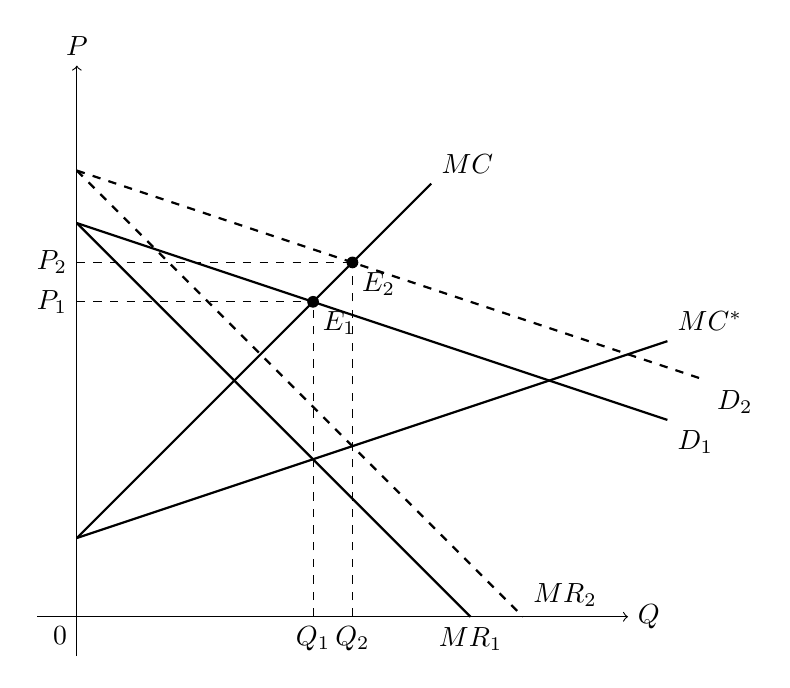
\begin{tikzpicture}
        % Axes
        \draw[->] (-0.5,0) -- (7,0) node[right] {$Q$}; % Horizontal axis
        \draw[->] (0,-0.5) -- (0,7) node[above] {$P$}; % Vertical axis
    
        % Demand Curve (D_1) - passes through (0,5), (3,4), and (7.5,2.5)
        \draw[thick] (0,5) -- (7.5,2.5) node[below right] {$D_1$};
    
        % Marginal Revenue (MR_1) - passes through (0,5), (3,2), and (5,0)
        \draw[thick] (0,5) -- (5,0) node[below] {$MR_1$};
    
        % Supply Curve under competition (S^c) - passes through (0,1), (3,4), and (4.5,5.5)
        \draw[thick] (0,1) -- (4.5,5.5) node[above right] {$MC$};
    
        % Supply Curve under monopoly (S^m) - passes through (0,1), (3,2), and (7.5,3.5)
        \draw[thick] (0,1) -- (7.5,3.5) node[above right] {$MC^{*}$};
    
        % Equilibrium point (E_1) - intersection of D_1 and S^c at (3,4)
        \node[circle, fill, inner sep=1.5pt] (E1) at (3,4) {};
        \node[below right] at (E1) {$E_1$};
    
    
        % Equilibrium point (E_2) - intersection of D_1 and S^c at (7/2,9/2)
        \node[circle, fill, inner sep=1.5pt] (E2) at (7/2,9/2) {};
        \node[below right] at (E2) {$E_2$};
    
        % Shifted Demand Curve (D_1 shifted)
        \draw[thick, dashed] (0,34/6) -- (8,3) node[below right] {$D_2$};
        
        % Shifted MR (MR_1 shifted)
        \draw[thick, dashed] (0,34/6) -- (34/6,0) node[above right] {$MR_2$};
        
        % Dashed lines for price and quantity
        \draw[dashed] (3,0) -- (3,4);
        \draw[dashed] (0,4) -- (3,4);
    
        \draw[dashed] (0,9/2) -- (7/2,9/2);
        \draw[dashed] (7/2,0) -- (7/2,9/2);
    
        % Additional labels
        \node[below left] at (0,0) {0};
        \node[left] at (0,4) {$P_1$};
        \node[below] at (3,0) {$Q_1$};
    
        \node[left] at (0,9/2) {$P_2$};
        \node[below] at (7/2,0) {$Q_2$};
    \end{tikzpicture}
    \end{center}
    \caption{The illustration of the non-identification result}
    \label{fig:bresnahan_non_identification}
    \vspace{2mm}
    \footnotesize
    Note: $MC$ is the marginal cost rationalized by the perfect competition, and $MC^{*}$ is the marginal cost rationalized by the perfect competition. $\beta_c = \beta_m + \alpha_1$ holds.
    The perfect competition and the monopoly rationalize the equilibrium point $E_1$. The shift in the demand does not help because the new equilibrium $E_2$ still are rationalized by both models.
\end{figure}


Let's investigate the same model with Lau's argument.
As Figure \ref{fig:bresnahan_non_identification} shows, the demand function and the marginal revenue with $\theta = 1$ have different slopes.
$MC$ and $MC^{*}$ are also different in the slope.
\begin{align}
    (1+\theta) \frac{\partial P}{\partial Q}(Q, X^d) + \theta \frac{\partial^2 P}{\partial Q^2}(Q, X^d) Q  - \frac{\partial MC}{\partial Q}(Q, X^s) = -\alpha_1(1 + \theta)   - \beta_1.
\end{align}
Due to the assumption on the marginal cost parameter between $MC$ and $MC^{*}$,
\begin{align}
    \lambda(X^{d}, X^{s}) = \frac{-2\alpha_1  - \beta_1^{*}}{-\alpha_1  - \beta_1} =   \frac{-2\alpha_1  -\beta_1 + \alpha_1}{-\alpha_1  - \beta_1} = 1.
\end{align}

The numerator of \eqref{eq:derivative_q_x_d} is given by
\begin{align}
    \frac{\partial P}{\partial X^{d}}(Q, X^{d}) + \theta\frac{\partial^2 P}{\partial X^{d}\partial Q}(Q, X^{d})Q   = \alpha_2
\end{align}
and the numerator of \eqref{eq:derivative_q_x_s} is given by
\begin{align}
    \frac{\partial MC}{\partial X^{s}}(Q, X^{s}) = \beta_2.
\end{align}
Then, \eqref{eq:derivative_q_x_d} and \eqref{eq:derivative_q_x_s} are 
\begin{align}
    \frac{\partial h}{\partial X^{d}}(Q, X^{d}) = \frac{\partial h^{*}}{\partial X^{d}}(Q, X^{d})  = \frac{\alpha_2}{\alpha_1 + \beta_1},\\
    \frac{\partial h}{\partial X^{s}}(Q, X^{s}) = \frac{\partial h^{*}}{\partial X^{s}}(Q, X^{s})  =-\frac{\beta_2}{\alpha_1 + \beta_1}.
\end{align}
which implies that observable equivalence holds for any $X^d$ and $X^s$.


By applying Lemma \ref{lemma_1_GU}, we can say that there is a transformation $T$ such that
\begin{align}
    P(Q, X^d) + \frac{\partial P}{\partial Q}(Q, X^d) Q & = T(P(Q, X^d), Q)\\
    MC^{*}(Q, X^s) &= T(MC(Q, X^s), Q).
\end{align}
In this case, consider the following transformation:
\begin{align}
    T(x, Q) = x + \alpha_1(\theta - \theta^{*})Q.
\end{align}
Then, we have
\begin{align}
    T(MC(Q, X^s), Q) & =  \beta_0 + \beta_1 Q + \beta_2 X^s + \alpha_1(\theta - \theta^{*})Q\\
    & = \beta_0^{*} + \beta_1^{*} Q + \beta_2^{*} X^s\\
    & = MC^{*}(Q, X^s).
\end{align}
and
\begin{align}
    T\left(P(Q, X^d) + \theta \frac{\partial P}{\partial Q}(Q, X^d) Q, Q\right) & = P(Q, X^d) -\theta \alpha_1 Q +  \alpha_1(\theta - \theta^{*})Q\\ 
    & = P(Q, X^d) - \theta^{*} \alpha_1 Q  \\
    & = P(Q, X^d) + \theta^{*} \frac{\partial P}{\partial Q}(Q, X^d) Q.
\end{align}

\subsection{The log-linear model}
The simplified version of our example is the following:
\begin{align}
    P & = \exp(\alpha_0) Q^{-\alpha_1} (X^{d})^{\alpha_2}, \\
    MC & = \exp(\beta_0) Q^{\beta_1} (X^{s})^{\beta_2}.
\end{align}
and hence, the marginal revenue is
\begin{align}
    MR = (1- \theta\alpha_1)\exp(\alpha_0) Q^{-\alpha_1} (X^{d})^{\alpha_2}
\end{align}
Take the logarithm of the demand and the marginal revenue, we have
\begin{align}
    \log P & = \alpha_0 -\alpha_1 \log Q + \alpha_2 \log X^{d},\\
    \log MR& = \log (1 -\theta\alpha_1) + \alpha_0 -\alpha_1 \log Q + \alpha_2 \log X^{d}.
\end{align}
The logarithm of the marginal cost is given by
\begin{align}
    \log MC & = \beta_0 + \beta_1 \log Q + \beta_2 \log X^{s}.
\end{align}
The intersection of the marginal revenue and the marginal cost gives the equilibrium log quantity;
\begin{align}
    \log Q &= \frac{ \log (1 - \theta \alpha_1) + \alpha_0 - \beta_0 +\alpha_2 \log X^{d} - \beta_2 \log X^{s}}{\alpha_1 + \beta_1}.
\end{align}
Thus, the equilibrium quantity is given by
\begin{align}
    Q^e &= \left[(1 - \theta \alpha_1)\exp(\alpha_0 - \beta_0)\right]^{\frac{1}{\alpha_1 + \beta_1}} (X^{d})^{\frac{\alpha_2}{\alpha_1 + \beta_1}} (X^{s})^{\frac{\beta_2}{\alpha_1 + \beta_1}}.
\end{align}
Based on the equilibrium quantity, consider an alternative model where the marginal cost function is defined as
\begin{align}
    MC^{*}(Q, X^{s}) = \exp(\beta_0^*) Q^{\beta_1^*} (X^{s})^{\beta_2^*}
\end{align}
where 
\begin{align}
    \beta_0^* = \beta_0 + \log\left(\frac{1-\theta^*\alpha_1}{1 - \theta\alpha_1}\right),\quad\beta_1^* = \beta_1,\quad \beta_2^* = \beta_2.
\end{align}
Then, between the true model and the alternative model, we have 
\begin{align}
    \lambda(Q, X^{s}) & = \frac{(1 -\theta\alpha_1)\alpha_1 \exp(\alpha_0) Q^{-\alpha_1 - 1}(X^{d})^{\alpha_2} - \beta_1 \exp(\beta_0)Q^{\beta_1-1} (X^{s})^{\beta_2}}{(1 -\theta^{*}\alpha_1)\alpha_1 \exp(\alpha_0) Q^{-\alpha_1 - 1}(X^{d})^{\alpha_2} - \beta_1^{*} \exp(\beta_0^{*})Q^{\beta_1^{*}-1} (X^{s})^{\beta_2^{*}}} \\
    & = \frac{(1 -\theta\alpha_1)\alpha_1 \exp(\alpha_0) Q^{-\alpha_1 - 1}(X^{d})^{\alpha_2} - \beta_1 \exp(\beta_0)Q^{\beta_1-1} (X^{s})^{\beta_2}}{(1 -\theta^{*}\alpha_1)\alpha_1 \exp(\alpha_0) Q^{-\alpha_1 - 1}(X^{d})^{\alpha_2} - \beta_1 \exp(\beta_0)\left(\frac{1-\theta^*\alpha_1}{1 - \theta\alpha_1}\right)   Q^{\beta_1-1} (X^{s})^{\beta_2}} \\
    & = \left(\frac{1-\theta^*\alpha_1}{1 - \theta\alpha_1}\right).
\end{align}
Thus, the transformation can be defined as
\begin{align}
    T(x, Q) = \frac{1 - \theta^* \alpha_1}{1 - \theta \alpha_1}x.
\end{align}
In fact, under the transformation, we have
\begin{align}
    T\left(P(Q, X^{d}) + \theta \frac{\partial P}{\partial Q}(Q, X^{d}) Q, Q\right)
    &= \frac{1 - \theta^*\alpha_1}{1- \theta\alpha_1} (1 - \theta\alpha_1)\exp(\alpha_0) Q^{-\alpha_1} (X^{d})^{\alpha_2}\\
    & = (1 - \theta^{*}\alpha_1)\exp(\alpha_0) Q^{-\alpha_1} (X^{d})^{\alpha_2}\\
    &= P(Q, X^{d}) + \theta^{*} \frac{\partial P}{\partial Q}(Q, X^{d}) Q
\end{align}
and
\begin{align}
    T\left(MC(Q, X^{s}), Q\right) &= \frac{1 - \theta^*\alpha_1}{1- \theta\alpha_1}\exp(\beta_0) Q^{\beta_1} (X^{s})^{\beta_2}\\
    &= \exp\left(\beta_0 + \log\left(\frac{1 - \theta^*\alpha_1}{1- \theta\alpha_1}\right)\right) Q^{\beta_1} (X^{s})^{\beta_2}\\
    &= MC^{*}(Q, X^{s}).
\end{align}
Thus, $(\theta, MC)$ and $(\theta^{*}, MC^{*})$ are observably equivalent.


\end{document}